\documentclass[11pt]{article}
\usepackage{graphicx}
\usepackage{amssymb}
\usepackage{color}

\pagestyle{empty}

\textwidth = 6.5 in
\textheight = 9 in
\oddsidemargin = 0.0 in
\evensidemargin = 0.0 in
\topmargin = 0.0 in
\headheight = 0.0 in
\headsep = 0.0 in
\parskip = 0.2in
\parindent = 0.0in


\begin{document}
{\large {\bf CMPT 202 - Greedy Coins Game}} 

There is a single row of $n$ coins with values $V_1$, $V_2$, ... $V_n$ where $n$ is even. A game is played against an opponent by alternating turns. For each turn, a player selects either the first or last coin from the row, removes it from the row, and receives the value of that coin. The object of the game is to claim the largest amount of money in coins.

As an example, the first player (Alice) can choose either the 3 or the 2. 

\begin{figure}[h]
\centerline {
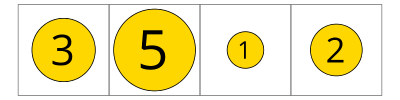
\includegraphics[width=3in]{img-1.png}
}

\end{figure}

Let's assume she chooses the 3 as it has a larger value. The coins now appear as

\begin{figure}[h]
\centerline {
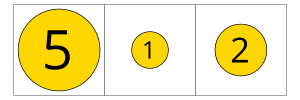
\includegraphics[width=3in]{img-2.png}
}

\end{figure}

The second player (Bob) may choose either the 5 or the 2, and will choose 5 as it is larger. We now have two remaining coins:

\begin{figure}[h]
\centerline {
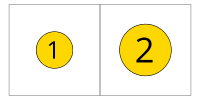
\includegraphics[width=2in]{img-3.png}
}

\end{figure}

Alice will choose the 2, and Bob will choose 1. The final score is Alice = 5 and Bob = 6.

So as you can see, having the first player initially choosing the highest-valued coin (known as a {\it greedy} algorithm) may not be an optimal strategy.  Instead, Alice should have initially chosen 2. Bob would have then chosen 3. Alice next chooses 5 and Bob chooses 1. Alice wins with a score of 7.

Design an algorithm that ensures the player that goes first can never lose. Rather, the first player will either win or tie. The goal of the game is not to get the optimal value of coins, but rather ensure the first player {\it never} loses. 

A few possible test cases (winning value is bold-faced.) 

10 5 {\bf 10} \\
3 5 1 2 {\bf 7} \\
8 9 8 5 5 0 {\bf 21} \\
83 50 14 11 39 79 1 25 {\bf 165}

\newpage

{\large {\bf Red-Blue Strategy}} 

One possible strategy to ensure the computer never loses is known  as {\it red-blue} whereby each coin is assigned the color {\color{red}red} or {\color{blue}blue}. The color of each coin alternates, beginning with {\color{red}red}. For example, the coins 

83 50 14 11 39 79 1 25

would be assigned the colors

{\color{red}83} {\color{blue}50} {\color{red}14} {\color{blue}11} {\color{red}39} {\color{blue}79} {\color{red}1} {\color{blue}25}

Before the game proceeds, the computer adds up the possible scores for coins colored red and coins colored blue. Which in this case is

{\color{red}red = 137} \\
{\color{blue}blue = 165}

The best strategy is to choose the color coins that have the highest value. In this case, if the computer chooses all blue coins, they will win. For all cases, the computer will always either tie or win, and never lose. (Consider how a tie is possible.)

Using different examples, familiarize yourself with this strategy.

Next, remembering that the computer gets to go first and there is always an even number of coins, design an algorithm that allows the computer to always select the highest valued coins using the red-blue strategy.


 \end{document}
